
\subsection{Velocity field}

The velocity field for the Smith-Hutton case is given by $\vb{v} = 2 y (1 - x^2)
\vb{i} - 2 x (1 - y^2) \vb{j}$. It verifies the incompressibility condition
since it is divergence--free, \ie $\div{\vb{v}} = 0$. The only points where
$\vb{v}$ vanishes are $(0,0)$ and $(\pm 1, \pm 1)$. In the case of $L < 1$, only
$(0,0)$ belongs to $\overline{\Omega}$. Otherwise, $(0,0)$, $(-1,1)$ and $(1,1)$
the first three points belong to $\overline{\Omega}$. 

Recall that the
stream function is a mapping $\psi \colon U \subset \real^2 \to \real$, where
$U$ is some open subset of $\real^2$ containing $\Omega$, such that
\begin{equation*}
	u = \pdv{\psi}{y}, \quad
	v = -\pdv{\psi}{x}
\end{equation*}
By choosing $u$ and $v$ to be the components of the velocity field $\vb{v}$ and
integrating, one finds the function $\psi(x,y) = x^2 + y^2 (1 - x^2) + C$ where
$C \in \real$ is a constant. Since the constant vanishes when differentiating,
we may choose $C = -1$ so that we obtain the more nice looking
\begin{equation*}
	\psi(x,y) = -(1 - x^2)(1 - y^2)
\end{equation*}

Henceforth we will assume $L = 1 \ \meter$. In order to find the analytical
solution to problem \eqref{eq:smith_hutton_cauchy_problem} when $\Gamma = 0$, it
will be useful to know how the streamlines are. Recall that the streamlines are
defined as the curves tangent to the vector field $\vb{v}$ at each point. If
$\alpha \colon I \subset \real \to \Omega$, $s \mapsto \alpha(s) = (x(s), y(s))$
is the parametrization of a curve in $\Omega$, then it is a streamline provided
it satisifes the following system of ODEs:
\begin{equation} \label{eq:velocity_smith_hutton_odes}
	\left\{
	\begin{aligned}
		x' &= 2 y (1 - x^2) \\
		y' &= - 2 x (1 - y^2)
	\end{aligned}
	\right.
\end{equation}
Equivalently, the streamlines are the curves with normal vector $\grad{\psi}$ at
every point. In order to find the streamlines, we can specify an initial
condition and then pose the corresponding initial value problem. Consider the
mapping $f \colon \real^2 \longrightarrow \real^2$ defined by
\begin{equation} \label{eq:smith_hutton_velocity_mapping}
	f(x,y) = 
	\begin{pmatrix}
		u(x,y) \\ v(x,y)
	\end{pmatrix} =
	\begin{pmatrix}
		2 y (1 - x^2) \\ - 2 x (1 - y^2)
	\end{pmatrix}
\end{equation}
Then the initial value problem for a streamline with initial condition $(x_0,y_0) \in \overline{\Omega}$ is
\begin{equation} \label{eq:vel_smith_hutton_ivp}
	\left\{
		\begin{aligned}
			\alpha' &= f(\alpha(s)) \\
			\alpha(0) &= (x_0, y_0)
		\end{aligned}
	\right.
\end{equation}

\begin{prop} \label{prop:existence_uniqueness_streamlines}
	The solution to the initial value problem \eqref{eq:vel_smith_hutton_ivp}
	exists and is unique for every $(x_0, y_0) \in \overline{\Omega}$.
\end{prop}
\begin{proof}
	Let $U = B(0,2L)$, thus $\overline{\Omega} \subset U$. Since both $u$ and
	$v$ are $\mathcal{C}^\infty(\real^2)$ functions, $f$ is
	$\mathcal{C}^\infty(\real^2)$. The restriction of $f$ to $\overline{U}$ is,
	in particular, a $\mathcal{C}^1(\overline{U})$ mapping. By theorem
	\ref{teo:c1_function_implies_lipschitz}, $f$ is Lipschitz on $\overline{U}$.
	Now by the Picard--Lindelöf theorem (Theorem \ref{teo:picard_lindelof}) we
	deduce the existence and uniqueness of solution to
	\eqref{eq:vel_smith_hutton_ivp}.
\end{proof}

Finding the explicit solution to \eqref{eq:vel_smith_hutton_ivp} might be
difficult as the system is non--linear. Nonetheless we can solve it numerically
so as to find the appearance of the streamlines. This is precisely what has been
done to produce figure \eqref{fig:smith_hutton_N201_streamlines}. The RK4
algorithm was applied to the IVP \eqref{eq:vel_smith_hutton_ivp} for initial
conditions $x_0 = 0.10, \ 0.20, \ 0.30, \ 0.40, \ 0.50, \ 0.60, \ 0.70, \ 0.80,
\ 0.90, \ 0.99 \ \meter$ and $y_0 = 0$.

\begin{figure}[ht]
	\centering
	%	\fbox{% GNUPLOT: LaTeX picture with Postscript
\begingroup
  % Encoding inside the plot.  In the header of your document, this encoding
  % should to defined, e.g., by using
  % \usepackage[cp1252,<other encodings>]{inputenc}
  \inputencoding{cp1252}%
  \makeatletter
  \providecommand\color[2][]{%
    \GenericError{(gnuplot) \space\space\space\@spaces}{%
      Package color not loaded in conjunction with
      terminal option `colourtext'%
    }{See the gnuplot documentation for explanation.%
    }{Either use 'blacktext' in gnuplot or load the package
      color.sty in LaTeX.}%
    \renewcommand\color[2][]{}%
  }%
  \providecommand\includegraphics[2][]{%
    \GenericError{(gnuplot) \space\space\space\@spaces}{%
      Package graphicx or graphics not loaded%
    }{See the gnuplot documentation for explanation.%
    }{The gnuplot epslatex terminal needs graphicx.sty or graphics.sty.}%
    \renewcommand\includegraphics[2][]{}%
  }%
  \providecommand\rotatebox[2]{#2}%
  \@ifundefined{ifGPcolor}{%
    \newif\ifGPcolor
    \GPcolortrue
  }{}%
  \@ifundefined{ifGPblacktext}{%
    \newif\ifGPblacktext
    \GPblacktextfalse
  }{}%
  % define a \g@addto@macro without @ in the name:
  \let\gplgaddtomacro\g@addto@macro
  % define empty templates for all commands taking text:
  \gdef\gplbacktext{}%
  \gdef\gplfronttext{}%
  \makeatother
  \ifGPblacktext
    % no textcolor at all
    \def\colorrgb#1{}%
    \def\colorgray#1{}%
  \else
    % gray or color?
    \ifGPcolor
      \def\colorrgb#1{\color[rgb]{#1}}%
      \def\colorgray#1{\color[gray]{#1}}%
      \expandafter\def\csname LTw\endcsname{\color{white}}%
      \expandafter\def\csname LTb\endcsname{\color{black}}%
      \expandafter\def\csname LTa\endcsname{\color{black}}%
      \expandafter\def\csname LT0\endcsname{\color[rgb]{1,0,0}}%
      \expandafter\def\csname LT1\endcsname{\color[rgb]{0,1,0}}%
      \expandafter\def\csname LT2\endcsname{\color[rgb]{0,0,1}}%
      \expandafter\def\csname LT3\endcsname{\color[rgb]{1,0,1}}%
      \expandafter\def\csname LT4\endcsname{\color[rgb]{0,1,1}}%
      \expandafter\def\csname LT5\endcsname{\color[rgb]{1,1,0}}%
      \expandafter\def\csname LT6\endcsname{\color[rgb]{0,0,0}}%
      \expandafter\def\csname LT7\endcsname{\color[rgb]{1,0.3,0}}%
      \expandafter\def\csname LT8\endcsname{\color[rgb]{0.5,0.5,0.5}}%
    \else
      % gray
      \def\colorrgb#1{\color{black}}%
      \def\colorgray#1{\color[gray]{#1}}%
      \expandafter\def\csname LTw\endcsname{\color{white}}%
      \expandafter\def\csname LTb\endcsname{\color{black}}%
      \expandafter\def\csname LTa\endcsname{\color{black}}%
      \expandafter\def\csname LT0\endcsname{\color{black}}%
      \expandafter\def\csname LT1\endcsname{\color{black}}%
      \expandafter\def\csname LT2\endcsname{\color{black}}%
      \expandafter\def\csname LT3\endcsname{\color{black}}%
      \expandafter\def\csname LT4\endcsname{\color{black}}%
      \expandafter\def\csname LT5\endcsname{\color{black}}%
      \expandafter\def\csname LT6\endcsname{\color{black}}%
      \expandafter\def\csname LT7\endcsname{\color{black}}%
      \expandafter\def\csname LT8\endcsname{\color{black}}%
    \fi
  \fi
    \setlength{\unitlength}{0.0500bp}%
    \ifx\gptboxheight\undefined%
      \newlength{\gptboxheight}%
      \newlength{\gptboxwidth}%
      \newsavebox{\gptboxtext}%
    \fi%
    \setlength{\fboxrule}{0.5pt}%
    \setlength{\fboxsep}{1pt}%
    \definecolor{tbcol}{rgb}{1,1,1}%
\begin{picture}(7370.00,3968.00)%
    \gplgaddtomacro\gplbacktext{%
      \csname LTb\endcsname%%
      \put(814,719){\makebox(0,0)[r]{\strut{}0.0}}%
      \put(814,1234){\makebox(0,0)[r]{\strut{}0.2}}%
      \put(814,1748){\makebox(0,0)[r]{\strut{}0.4}}%
      \put(814,2263){\makebox(0,0)[r]{\strut{}0.6}}%
      \put(814,2777){\makebox(0,0)[r]{\strut{}0.8}}%
      \put(814,3292){\makebox(0,0)[r]{\strut{}1.0}}%
      \put(946,499){\makebox(0,0){\strut{}-1.0}}%
      \put(2233,499){\makebox(0,0){\strut{}-0.5}}%
      \put(3520,499){\makebox(0,0){\strut{}0.0}}%
      \put(4806,499){\makebox(0,0){\strut{}0.5}}%
      \put(6093,499){\makebox(0,0){\strut{}1.0}}%
    }%
    \gplgaddtomacro\gplfronttext{%
      \csname LTb\endcsname%%
      \put(209,2005){\rotatebox{-270}{\makebox(0,0){\strut{}$y \ (\mathrm{m})$}}}%
      \put(3519,169){\makebox(0,0){\strut{}$x \ (\mathrm{m})$}}%
      \csname LTb\endcsname%%
      \put(6611,719){\makebox(0,0)[l]{\strut{}0.0}}%
      \put(6611,1362){\makebox(0,0)[l]{\strut{}0.5}}%
      \put(6611,2005){\makebox(0,0)[l]{\strut{}1.0}}%
      \put(6611,2648){\makebox(0,0)[l]{\strut{}1.5}}%
      \put(6611,3292){\makebox(0,0)[l]{\strut{}2.0}}%
      \put(7073,2005){\rotatebox{-270}{\makebox(0,0){\strut{}$\phi$}}}%
      \put(3519,3622){\makebox(0,0){\strut{}\textbf{Smith--Hutton case} $(\mathrm{Pe} = 10^{2})$}}%
    }%
    \gplbacktext
    \put(0,0){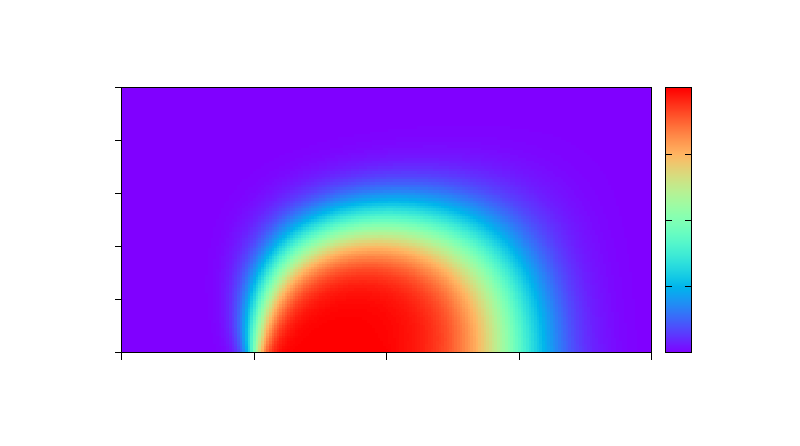
\includegraphics[width={368.50bp},height={198.40bp}]{figures/case_smith_hutton/smith_hutton_N201_Pe1.0e+02}}%
    \gplfronttext
  \end{picture}%
\endgroup
}
	% GNUPLOT: LaTeX picture with Postscript
\begingroup
  % Encoding inside the plot.  In the header of your document, this encoding
  % should to defined, e.g., by using
  % \usepackage[cp1252,<other encodings>]{inputenc}
  \inputencoding{cp1252}%
  \makeatletter
  \providecommand\color[2][]{%
    \GenericError{(gnuplot) \space\space\space\@spaces}{%
      Package color not loaded in conjunction with
      terminal option `colourtext'%
    }{See the gnuplot documentation for explanation.%
    }{Either use 'blacktext' in gnuplot or load the package
      color.sty in LaTeX.}%
    \renewcommand\color[2][]{}%
  }%
  \providecommand\includegraphics[2][]{%
    \GenericError{(gnuplot) \space\space\space\@spaces}{%
      Package graphicx or graphics not loaded%
    }{See the gnuplot documentation for explanation.%
    }{The gnuplot epslatex terminal needs graphicx.sty or graphics.sty.}%
    \renewcommand\includegraphics[2][]{}%
  }%
  \providecommand\rotatebox[2]{#2}%
  \@ifundefined{ifGPcolor}{%
    \newif\ifGPcolor
    \GPcolortrue
  }{}%
  \@ifundefined{ifGPblacktext}{%
    \newif\ifGPblacktext
    \GPblacktextfalse
  }{}%
  % define a \g@addto@macro without @ in the name:
  \let\gplgaddtomacro\g@addto@macro
  % define empty templates for all commands taking text:
  \gdef\gplbacktext{}%
  \gdef\gplfronttext{}%
  \makeatother
  \ifGPblacktext
    % no textcolor at all
    \def\colorrgb#1{}%
    \def\colorgray#1{}%
  \else
    % gray or color?
    \ifGPcolor
      \def\colorrgb#1{\color[rgb]{#1}}%
      \def\colorgray#1{\color[gray]{#1}}%
      \expandafter\def\csname LTw\endcsname{\color{white}}%
      \expandafter\def\csname LTb\endcsname{\color{black}}%
      \expandafter\def\csname LTa\endcsname{\color{black}}%
      \expandafter\def\csname LT0\endcsname{\color[rgb]{1,0,0}}%
      \expandafter\def\csname LT1\endcsname{\color[rgb]{0,1,0}}%
      \expandafter\def\csname LT2\endcsname{\color[rgb]{0,0,1}}%
      \expandafter\def\csname LT3\endcsname{\color[rgb]{1,0,1}}%
      \expandafter\def\csname LT4\endcsname{\color[rgb]{0,1,1}}%
      \expandafter\def\csname LT5\endcsname{\color[rgb]{1,1,0}}%
      \expandafter\def\csname LT6\endcsname{\color[rgb]{0,0,0}}%
      \expandafter\def\csname LT7\endcsname{\color[rgb]{1,0.3,0}}%
      \expandafter\def\csname LT8\endcsname{\color[rgb]{0.5,0.5,0.5}}%
    \else
      % gray
      \def\colorrgb#1{\color{black}}%
      \def\colorgray#1{\color[gray]{#1}}%
      \expandafter\def\csname LTw\endcsname{\color{white}}%
      \expandafter\def\csname LTb\endcsname{\color{black}}%
      \expandafter\def\csname LTa\endcsname{\color{black}}%
      \expandafter\def\csname LT0\endcsname{\color{black}}%
      \expandafter\def\csname LT1\endcsname{\color{black}}%
      \expandafter\def\csname LT2\endcsname{\color{black}}%
      \expandafter\def\csname LT3\endcsname{\color{black}}%
      \expandafter\def\csname LT4\endcsname{\color{black}}%
      \expandafter\def\csname LT5\endcsname{\color{black}}%
      \expandafter\def\csname LT6\endcsname{\color{black}}%
      \expandafter\def\csname LT7\endcsname{\color{black}}%
      \expandafter\def\csname LT8\endcsname{\color{black}}%
    \fi
  \fi
    \setlength{\unitlength}{0.0500bp}%
    \ifx\gptboxheight\undefined%
      \newlength{\gptboxheight}%
      \newlength{\gptboxwidth}%
      \newsavebox{\gptboxtext}%
    \fi%
    \setlength{\fboxrule}{0.5pt}%
    \setlength{\fboxsep}{1pt}%
    \definecolor{tbcol}{rgb}{1,1,1}%
\begin{picture}(7370.00,3968.00)%
    \gplgaddtomacro\gplbacktext{%
      \csname LTb\endcsname%%
      \put(814,733){\makebox(0,0)[r]{\strut{}$0$}}%
      \put(814,1242){\makebox(0,0)[r]{\strut{}$0.2$}}%
      \put(814,1751){\makebox(0,0)[r]{\strut{}$0.4$}}%
      \put(814,2260){\makebox(0,0)[r]{\strut{}$0.6$}}%
      \put(814,2769){\makebox(0,0)[r]{\strut{}$0.8$}}%
      \put(814,3278){\makebox(0,0)[r]{\strut{}$1$}}%
      \put(1009,513){\makebox(0,0){\strut{}-1.0}}%
      \put(2282,513){\makebox(0,0){\strut{}-0.5}}%
      \put(3554,513){\makebox(0,0){\strut{}0.0}}%
      \put(4827,513){\makebox(0,0){\strut{}0.5}}%
      \put(6099,513){\makebox(0,0){\strut{}1.0}}%
    }%
    \gplgaddtomacro\gplfronttext{%
      \csname LTb\endcsname%%
      \put(209,2005){\rotatebox{-270}{\makebox(0,0){\strut{}$y \ (\mathrm{m})$}}}%
      \put(3554,183){\makebox(0,0){\strut{}$x \ (\mathrm{m})$}}%
      \csname LTb\endcsname%%
      \put(6612,733){\makebox(0,0)[l]{\strut{}0.0}}%
      \put(6612,1369){\makebox(0,0)[l]{\strut{}0.5}}%
      \put(6612,2005){\makebox(0,0)[l]{\strut{}1.0}}%
      \put(6612,2641){\makebox(0,0)[l]{\strut{}1.5}}%
      \put(6612,3278){\makebox(0,0)[l]{\strut{}2.0}}%
      \put(7074,2005){\rotatebox{-270}{\makebox(0,0){\strut{}$\norm{\vb{v}} \ (\mathrm{m} / \mathrm{s})$}}}%
      \put(3554,3608){\makebox(0,0){\strut{}\textbf{Smith--Hutton case -- Velocity field}}}%
    }%
    \gplbacktext
    \put(0,0){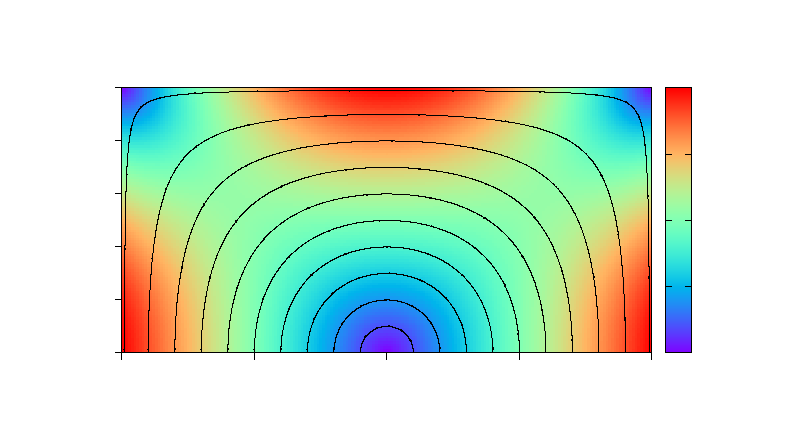
\includegraphics[width={368.50bp},height={198.40bp}]{figures/case_smith_hutton/smith_hutton_N201_streamlines}}%
    \gplfronttext
  \end{picture}%
\endgroup

	\captionsetup{width=0.75\textwidth}
	\caption{Norm of the Smith--Hutton velocity field and streamlines for $x_0 =
	0.10, \ 0.20, \ 0.30, \ 0.40, \ 0.50, \ 0.60, \ 0.70, \ 0.80, \ 0.90$ and
	$0.99 \ \meter$. The vectors tangent to the streamlines are normalized and
	then scaled down by a factor of $\sqrt{2}/50$.}
	\label{fig:smith_hutton_N201_streamlines}
\end{figure}